\chapter{\textbf{Design og utforming}}

\subsection{\textbf{Universell utforming}}
Universell utforming handler om å utforme omgivelsene slik at vi tar hensyn til variasjonen i funksjonsevne hos innbyggerne, inkludert personer med nedsatt funksjonsevne.\cite{digiuniversell} Hensikten er å kunne nå alle målgruppene gjennom en og samme løsning. Forskriften om universell utforming av IKT-løsninger stiller krav om at nettsider må oppfylle 35 av 61 suksesskriterier i “Retningslinjer for tilgjengelig webinnhold" \cite{digiwcag}. Mobilapplikasjonen vi har utviklet er omfattet da den må laste ned informasjon fra internett for å fungere.

Universell utforming er mer enn bare å tilrettelegge for mennesker med funksjonsnedsetting, men også eksempelvis mennesker med annet morsmål, lite domenekunnskap, vanskeligheter for å bruke mobiltelefon og så videre. Det har vært viktig for oss å ikke bare tenke på universell utforming, men aktivt inkludere det underveis i prosessen.

Det kan være vanskelig å følge alle retningslinjene, men det er lettere gjort når man inkluderer det i hele prosessen. Mange av våre designvalg har vært i tråd med artikler og forskning gjort av Nielsen Norman Group, som ansees for å være en av verdens fremste på forskningsbasert universell utforming og UX. Eksempelvis kan vi nevne det som kalles for input steppers. Det vil si et inputfelt med tilhørende knapper for + og -. En av de sentrale funksjonalitetene i løsningen er å kunne telle antallet man har av en vare. Vi var derfor helt avhengig av en god brukeropplevelse og har gjennom flere iterasjoner og bruk av forskning fra Nielsen Norman Group\cite{nngsteppers} kommet frem til en god måte å telle på. Ved å kunne taste inn store tall på eksempelvis vekt og volum, men samtidig kunne trykke en eller to ganger på en vare det ikke finnes mange av gir vi brukeren to valg og forenkler prosessen (REFERANSE TIL FIGUR). Vi kommer tilbake til hvor intuitivt brukeren syntes dette var i kapittel 7 (LINK TIL KAPITTEL)

\begin{figure}[H] 
    \centering
    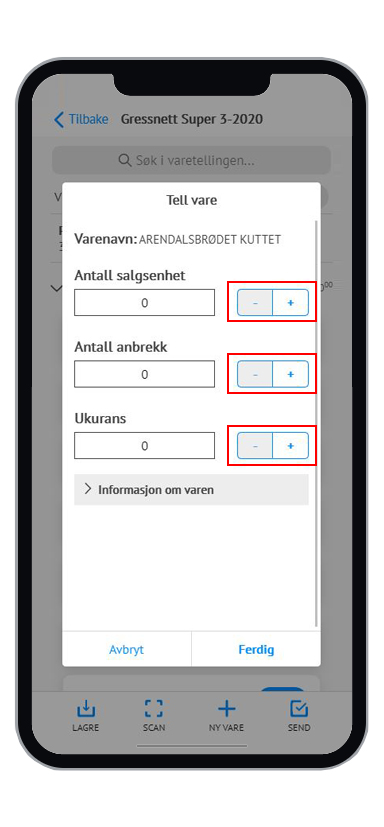
\includegraphics[width=75mm]{figures/Design-utforming/universell-utforming.jpg}
    \caption{Inputfelt (t.v). Input stepper markert i rød boks (t.h).}
\end{figure}
